% =====================================================================
%  Datasets_Report.tex -- stand-alone report on public datasets for
%  "Skin Cancer Detection Using Deep Learning".
%  Build: tectonic Datasets_Report.tex
% =====================================================================
\documentclass[10pt,a4paper]{article}
% =====================================================================
%  report_preamble.tex -- shared preamble for the stand-alone
%  Datasets and Algorithms reports (article class, A4).
% =====================================================================
\usepackage[T1]{fontenc}
\usepackage[utf8]{inputenc}
\usepackage{mathptmx}
\usepackage[a4paper,margin=2cm]{geometry}
\usepackage{amsmath,amssymb}
\usepackage{graphicx,xcolor}
\usepackage{tikz,pgfplots}
\pgfplotsset{compat=1.18}
\usetikzlibrary{positioning,arrows.meta,calc}
\usepackage{booktabs,array,multirow,tabularx,longtable}
\usepackage{pifont}
\providecommand{\checkmark}{\ding{51}}
\usepackage{enumitem}
\setlist{itemsep=1pt,topsep=3pt,parsep=0pt}
\usepackage[font=small,labelfont=bf]{caption}
\usepackage{float}
\usepackage{cite}
\usepackage{url}
\usepackage[colorlinks=true,linkcolor=hcBlue,citecolor=hcBlue,urlcolor=hcTeal]{hyperref}
\usepackage{titlesec}
\titleformat{\section}{\large\bfseries\color{hcBlue}}{\thesection}{0.6em}{}
\titleformat{\subsection}{\normalsize\bfseries}{\thesubsection}{0.6em}{}
\setlength{\parskip}{3pt}

% ---- Palette (colour-blind friendly) ----------------------------------
\definecolor{hcBlue}{HTML}{2166AC}
\definecolor{hcTeal}{HTML}{1B9E77}
\definecolor{hcOrange}{HTML}{D95F02}
\definecolor{hcPurple}{HTML}{7570B3}
\definecolor{hcRed}{HTML}{B2182B}
\definecolor{hcGray}{HTML}{6E6E6E}
\definecolor{boxBg}{HTML}{EEF3FA}

\pgfplotsset{
  hcaxis/.style={
    tick align=outside, tick pos=left, grid=major,
    major grid style={line width=0.2pt,draw=gray!30},
    axis line style={draw=gray!55},
    label style={font=\footnotesize},
    tick label style={font=\scriptsize},
    legend style={font=\scriptsize,draw=gray!40,fill=white,rounded corners=1pt},
    every node near coord/.append style={font=\tiny},
  }
}

\newcolumntype{L}[1]{>{\raggedright\arraybackslash}p{#1}}
\newcolumntype{Y}{>{\raggedright\arraybackslash}X}

% Highlight box for key take-aways
\newcommand{\keybox}[1]{%
  \par\smallskip\noindent\colorbox{boxBg}{\parbox{\dimexpr\linewidth-2\fboxsep}{\small #1}}\par\smallskip}


\title{\color{hcBlue}\bfseries Datasets for Skin Cancer Detection Using Deep Learning\\[4pt]
\large A Verified Survey of Public Datasets and a Recommended Combination}
\author{Project: Skin Cancer Detection Using Deep Learning\\
\small Companion document to the IEEE paper}
\date{September 2026}

\begin{document}
\maketitle
\thispagestyle{empty}

\begin{abstract}
\noindent This document surveys the public image datasets that are
suitable for a deep-learning skin cancer detection project. For each
dataset it reports the number of images, imaging modality, diagnostic
classes, available metadata, class balance, licence, and download
location. Image counts were checked against the official label files
or data papers. The document then recommends a combination of six
datasets that covers melanoma, basal cell carcinoma (BCC), and
squamous cell carcinoma (SCC), provides external and skin-tone-diverse
test sets, and avoids the duplicate images that inflate published
results.
\end{abstract}

\tableofcontents
\newpage

% =====================================================================
\section{Why Dataset Choice Matters}
A skin cancer classifier can only be as good as the data it learns
from. Three properties of public dermatology data strongly affect the
results a project reports:
\begin{enumerate}
  \item \textbf{Class imbalance.} Malignant lesions are rare. They
        make up 0.1\% of SLICE-3D, 1.8\% of ISIC~2020, and about 20\%
        of HAM10000 (Fig.~\ref{fig:prev}). A model that always predicts
        ``benign'' can still look accurate.
  \item \textbf{Duplicates and overlap.} Many lesions are photographed
        several times, and the ISIC collections re-use earlier data
        (e.g., ISIC~2019 contains HAM10000 and BCN20000). Removing
        duplicates reduced the best ISIC~2020 test AUC of 19 CNNs to
        0.80~\cite{cassidy2022isic}.
  \item \textbf{Limited diversity.} Across 21 open datasets, skin type
        was recorded for only 2.1\% of images and ethnicity for 1.3\%,
        and most images come from Europe, North America, and
        Oceania~\cite{wen2022}. Models trained on such data perform
        worse on darker skin~\cite{daneshjou2022ddi}.
\end{enumerate}

\keybox{\textbf{Key idea:} use one large dataset for training, and
\emph{different} datasets (another hospital, another camera, other skin
tones) for testing. A model that is good only on its own training
distribution is not ready for patients.}

% =====================================================================
\section{Summary of Public Datasets}
Table~\ref{tab:summary} lists the datasets reviewed. Malignant classes
are printed in bold. MEL = melanoma, BCC = basal cell carcinoma,
SCC = squamous cell carcinoma, AK/AKIEC = actinic keratosis /
intra-epithelial carcinoma, NV = nevus, BKL = benign keratosis,
DF = dermatofibroma, VASC = vascular lesion.

{\small
\renewcommand{\arraystretch}{1.2}
\begin{longtable}{@{}L{2.2cm} c r L{2.0cm} L{4.2cm} L{3.3cm}@{}}
\caption{Public skin-cancer datasets (counts from official label files or data papers).}\label{tab:summary}\\
\toprule
\textbf{Dataset} & \textbf{Year} & \textbf{Images} & \textbf{Modality} & \textbf{Classes} & \textbf{Metadata} \\
\midrule
\endfirsthead
\toprule
\textbf{Dataset} & \textbf{Year} & \textbf{Images} & \textbf{Modality} & \textbf{Classes} & \textbf{Metadata} \\
\midrule
\endhead
HAM10000~\cite{tschandl2018ham10000} & 2018 & 10{,}015 & Dermoscopic & 7: \textbf{MEL}, \textbf{BCC}, \textbf{AKIEC}, NV, BKL, DF, VASC & Age, sex, site, diagnosis method, lesion ID \\
ISIC~2016~\cite{gutman2016isic} & 2016 & 1{,}279 & Dermoscopic & Binary: \textbf{malignant} vs.\ benign & -- \\
ISIC~2017~\cite{codella2018isic2017} & 2017 & 2{,}750 & Dermoscopic & 3: \textbf{MEL}, seborrheic keratosis, NV & Approx.\ age, sex \\
ISIC~2018~\cite{codella2019isic2018} & 2018 & 2{,}594 (T1 train) & Dermoscopic & Task~1 masks; Task~3 = HAM10000 classes & As HAM10000 \\
ISIC~2019~\cite{gessert2020} & 2019 & 25{,}331 & Dermoscopic & 8: \textbf{MEL}, \textbf{BCC}, \textbf{SCC}, \textbf{AK}, NV, BKL, DF, VASC & Age, sex, site, lesion ID \\
BCN20000~\cite{hernandez2024bcn20000} & 2024 & 18{,}946 & Dermoscopic & 8 (as ISIC~2019) + out-of-distribution & Age, sex, site, lesion ID \\
ISIC~2020~\cite{rotemberg2021isic2020} & 2020 & 33{,}126 & Dermoscopic & Binary: \textbf{MEL} vs.\ benign & Patient ID, age, sex, site \\
SLICE-3D (ISIC~2024)~\cite{kurtansky2024slice3d} & 2024 & 401{,}059 & 3D total-body photo crops & Binary: \textbf{malignant} (MEL, BCC, SCC) vs.\ benign & Age, sex, site, lighting, lesion features \\
MILK10k (ISIC~2025)~\cite{tschandl2026milk10k} & 2026 & 10{,}480 & Paired clinical + dermoscopic & 11 incl.\ \textbf{BCC}, \textbf{SCC/KA}, \textbf{MEL}, \textbf{AKIEC} & Age, sex, site, skin tone \\
PH2~\cite{mendonca2013ph2} & 2013 & 200 & Dermoscopic & 3: \textbf{MEL}, atypical NV, common NV & Masks, dermoscopic criteria \\
Derm7pt~\cite{kawahara2019derm7pt} & 2019 & 1{,}011 cases & Clinical + dermoscopic & \textbf{MEL}, \textbf{BCC}, NV, SK, misc. & 7-point checklist, sex, site \\
PAD-UFES-20~\cite{pacheco2020padufes20} & 2020 & 2{,}298 & Smartphone & 6: \textbf{BCC}, \textbf{SCC}, \textbf{MEL}, ACK, SEK, NEV & 21 fields incl.\ Fitzpatrick \\
Fitzpatrick~17k~\cite{groh2021fitzpatrick17k} & 2021 & 16{,}577 & Clinical atlas & 114 conditions; \textbf{malignant} / benign / non-neoplastic & Fitzpatrick I--VI \\
DDI~\cite{daneshjou2022ddi} & 2022 & 656 & Clinical & Binary: \textbf{malignant} vs.\ benign (biopsy-proven) & Fitzpatrick groups \\
MED-NODE~\cite{giotis2015mednode} & 2015 & 170 & Clinical & \textbf{MEL} vs.\ NV & -- \\
Dermofit~\cite{ballerini2013dermofit} & 2013 & 1{,}300 & Clinical & 10 incl.\ \textbf{MEL}, \textbf{BCC}, \textbf{SCC}, \textbf{IEC} & -- (paid licence) \\
SCIN~\cite{ward2024scin} & 2024 & 10{,}408 & Self-taken smartphone & Mostly inflammatory / infectious conditions & Self-reported demographics, skin tone \\
\bottomrule
\end{longtable}
}

\begin{figure}[H]
\centering
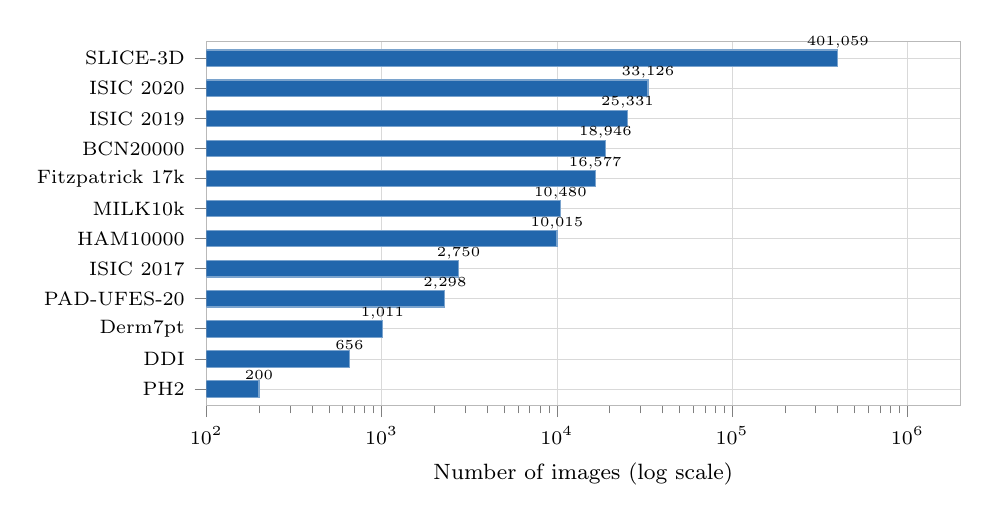
\begin{tikzpicture}
\begin{axis}[hcaxis,
  width=0.92\linewidth,height=6.2cm,
  xbar, bar width=6pt, bar shift=0pt,
  xmode=log, log basis x=10,
  xmin=100,xmax=2000000,
  ytick={1,...,12},
  yticklabels={PH2,DDI,Derm7pt,PAD-UFES-20,ISIC 2017,HAM10000,MILK10k,Fitzpatrick 17k,BCN20000,ISIC 2019,ISIC 2020,SLICE-3D},
  y tick label style={font=\scriptsize},
  xlabel={Number of images (log scale)},
  nodes near coords,
  point meta=explicit symbolic,
  enlarge y limits=0.05]
\addplot[fill=hcBlue,draw=hcBlue!60] coordinates {
 (200,1)[200] (656,2)[656] (1011,3)[1{,}011] (2298,4)[2{,}298] (2750,5)[2{,}750]
 (10015,6)[10{,}015] (10480,7)[10{,}480] (16577,8)[16{,}577] (18946,9)[18{,}946]
 (25331,10)[25{,}331] (33126,11)[33{,}126] (401059,12)[401{,}059]};
\end{axis}
\end{tikzpicture}
\caption{Dataset sizes (log scale). Derm7pt is counted in cases (each has clinical and dermoscopic images).}
\label{fig:sizes}
\end{figure}

% =====================================================================
\section{Class Balance and Malignant Prevalence}

\begin{figure}[H]
\centering
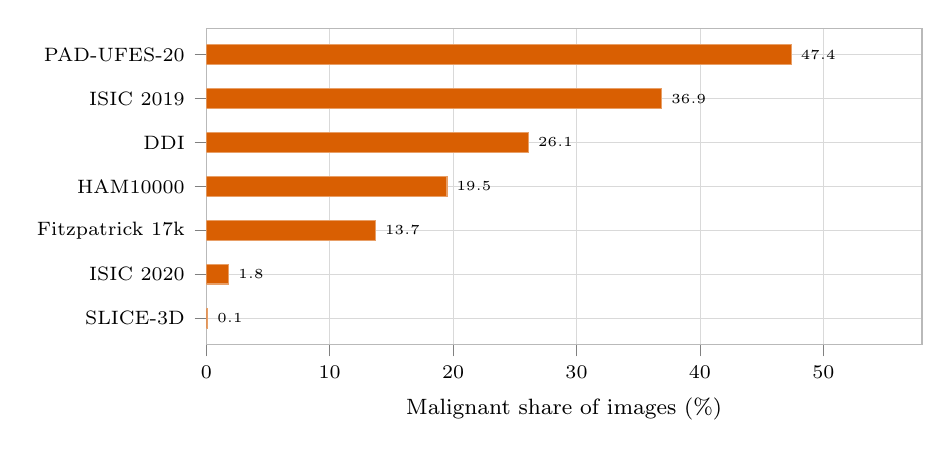
\begin{tikzpicture}
\begin{axis}[hcaxis,
  width=0.88\linewidth,height=5.6cm,
  xbar, bar width=7pt, bar shift=0pt,
  ytick={1,...,7},
  yticklabels={SLICE-3D,ISIC 2020,Fitzpatrick 17k,HAM10000,DDI,ISIC 2019,PAD-UFES-20},
  y tick label style={font=\scriptsize},
  xlabel={Malignant share of images (\%)},
  xmin=0,xmax=58, nodes near coords, enlarge y limits=0.1]
\addplot[fill=hcOrange,draw=hcOrange!60] coordinates {
 (0.1,1)(1.8,2)(13.7,3)(19.5,4)(26.1,5)(36.9,6)(47.4,7)};
\end{axis}
\end{tikzpicture}
\caption{Malignant share per dataset, computed from the official label files. HAM10000 and ISIC~2019 include the AKIEC/AK class. PAD-UFES-20 counts BCC, SCC, and MEL.}
\label{fig:prev}
\end{figure}

\begin{figure}[H]
\centering
\begin{minipage}{0.49\linewidth}
\centering
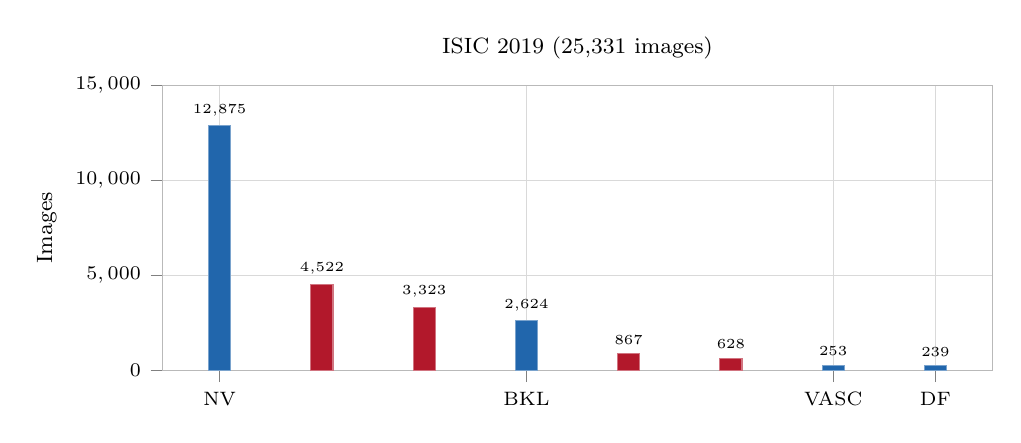
\begin{tikzpicture}
\begin{axis}[hcaxis,
  width=\linewidth,height=5.2cm,
  ybar, bar width=8pt, bar shift=0pt,
  symbolic x coords={NV,MEL,BCC,BKL,AK,SCC,VASC,DF},
  xtick=data, x tick label style={font=\scriptsize},
  ylabel={Images}, ymin=0,ymax=15000,
  scaled y ticks=false,
  yticklabel style={/pgf/number format/fixed,/pgf/number format/1000 sep={,}},
  nodes near coords, enlarge x limits=0.08,
  title={\footnotesize ISIC 2019 (25{,}331 images)}]
\addplot[fill=hcBlue,draw=hcBlue!60] coordinates {(NV,12875)(BKL,2624)(VASC,253)(DF,239)};
\addplot[fill=hcRed,draw=hcRed!60] coordinates {(MEL,4522)(BCC,3323)(AK,867)(SCC,628)};
\end{axis}
\end{tikzpicture}
\end{minipage}\hfill
\begin{minipage}{0.49\linewidth}
\centering
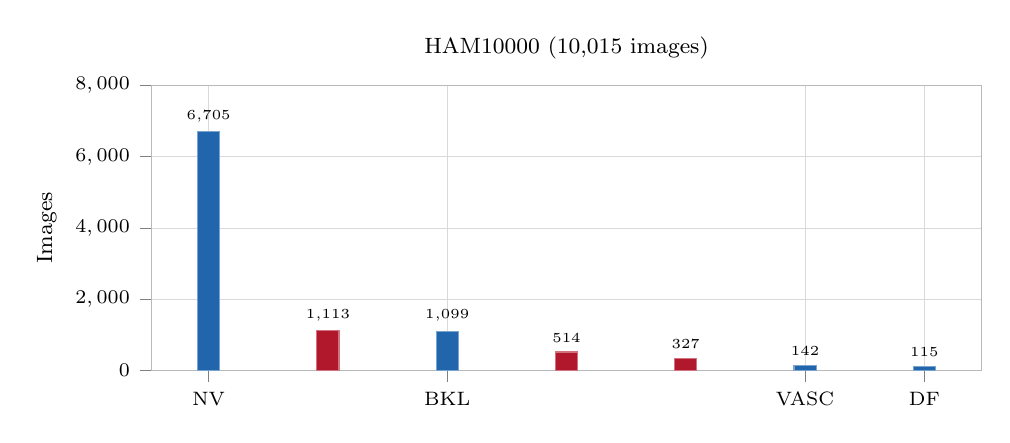
\begin{tikzpicture}
\begin{axis}[hcaxis,
  width=\linewidth,height=5.2cm,
  ybar, bar width=8pt, bar shift=0pt,
  symbolic x coords={NV,MEL,BKL,BCC,AKIEC,VASC,DF},
  xtick=data, x tick label style={font=\scriptsize},
  ylabel={Images}, ymin=0,ymax=8000,
  scaled y ticks=false,
  yticklabel style={/pgf/number format/fixed,/pgf/number format/1000 sep={,}},
  nodes near coords, enlarge x limits=0.08,
  title={\footnotesize HAM10000 (10{,}015 images)}]
\addplot[fill=hcBlue,draw=hcBlue!60] coordinates {(NV,6705)(BKL,1099)(VASC,142)(DF,115)};
\addplot[fill=hcRed,draw=hcRed!60] coordinates {(MEL,1113)(BCC,514)(AKIEC,327)};
\end{axis}
\end{tikzpicture}
\end{minipage}
\caption{Class distributions of ISIC~2019 and HAM10000 (red = malignant or pre-malignant). In ISIC~2019 the largest class is 54$\times$ the smallest.}
\label{fig:classes}
\end{figure}

\begin{figure}[H]
\centering
\begin{minipage}{0.49\linewidth}
\centering
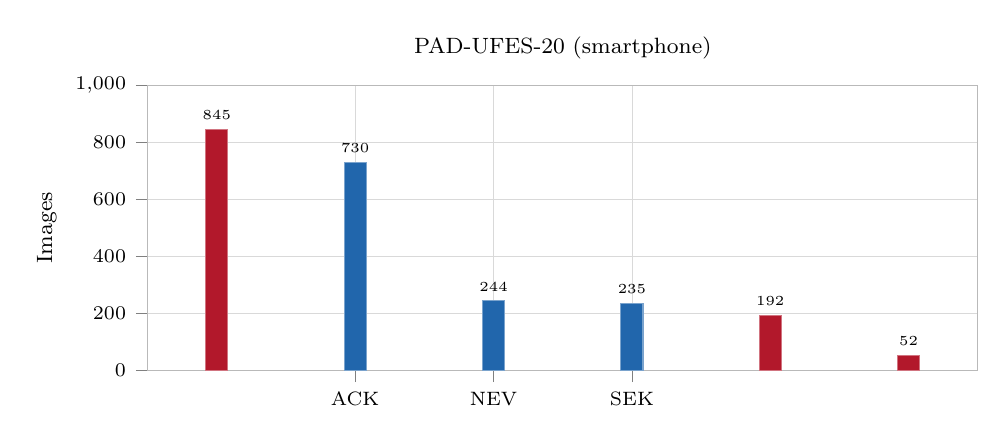
\begin{tikzpicture}
\begin{axis}[hcaxis,
  width=\linewidth,height=5.2cm,
  ybar, bar width=8pt, bar shift=0pt,
  symbolic x coords={BCC,ACK,NEV,SEK,SCC,MEL},
  xtick=data, x tick label style={font=\scriptsize},
  ylabel={Images}, ymin=0,ymax=1000,
  nodes near coords, enlarge x limits=0.1,
  title={\footnotesize PAD-UFES-20 (smartphone)}]
\addplot[fill=hcBlue,draw=hcBlue!60] coordinates {(ACK,730)(NEV,244)(SEK,235)};
\addplot[fill=hcRed,draw=hcRed!60] coordinates {(BCC,845)(SCC,192)(MEL,52)};
\end{axis}
\end{tikzpicture}
\end{minipage}\hfill
\begin{minipage}{0.49\linewidth}
\centering
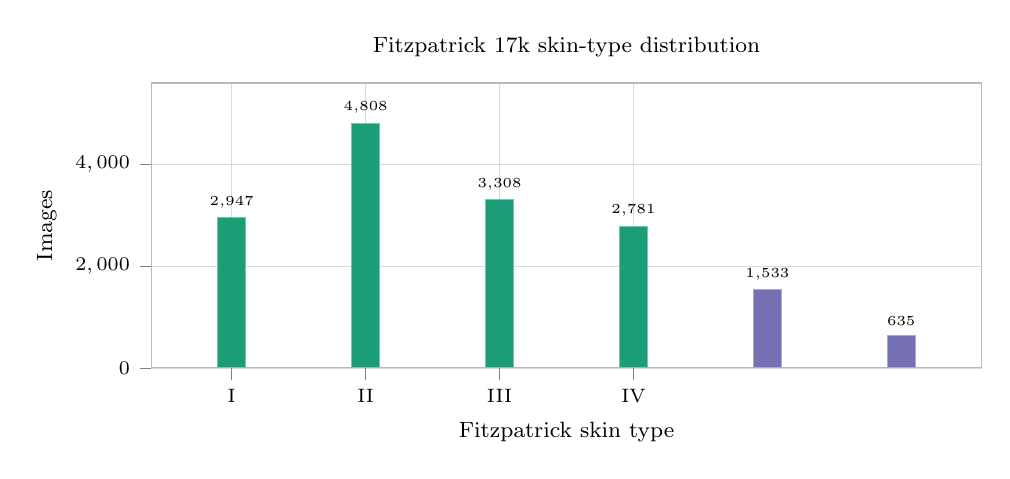
\begin{tikzpicture}
\begin{axis}[hcaxis,
  width=\linewidth,height=5.2cm,
  ybar, bar width=10pt, bar shift=0pt,
  symbolic x coords={I,II,III,IV,V,VI},
  xtick=data, x tick label style={font=\scriptsize},
  xlabel={Fitzpatrick skin type},
  ylabel={Images}, ymin=0,ymax=5600,
  scaled y ticks=false,
  yticklabel style={/pgf/number format/fixed,/pgf/number format/1000 sep={,}},
  nodes near coords, enlarge x limits=0.12,
  title={\footnotesize Fitzpatrick 17k skin-type distribution}]
\addplot[fill=hcTeal,draw=hcTeal!60] coordinates {(I,2947)(II,4808)(III,3308)(IV,2781)};
\addplot[fill=hcPurple,draw=hcPurple!60] coordinates {(V,1533)(VI,635)};
\end{axis}
\end{tikzpicture}
\end{minipage}
\caption{Left: PAD-UFES-20 classes (red = cancers; ACK is pre-malignant). Right: Fitzpatrick~17k skin types. Darker types V--VI (purple) make up only 13\% of images.}
\label{fig:pad}
\end{figure}

% =====================================================================
\section{Dataset Profiles}

\subsection{HAM10000}
\emph{10{,}015 dermoscopic images, 7 classes}~\cite{tschandl2018ham10000}.
Collected in Vienna and Queensland. More than half of the diagnoses are
confirmed by histopathology (5{,}340); the rest are confirmed by
follow-up, expert consensus, or confocal microscopy. It is the most
widely used benchmark and is identical to the ISIC~2018 Task~3 training
set. \textbf{Caution:} it has 7{,}470 unique lesions, so several images
share a lesion. Split by \texttt{lesion\_id}, not by image, to avoid
leakage. Licence: CC BY-NC 4.0.

\subsection{ISIC 2016, 2017, and 2018 Challenges}
These early ISIC challenge sets~\cite{gutman2016isic,codella2018isic2017,codella2019isic2018}
are small and dermoscopic. Their main value today is the
\textbf{lesion segmentation masks}: ISIC~2018 Task~1 provides 2{,}594
training, 100 validation, and 1{,}000 test images with expert masks.
ISIC~2017 adds a three-class task (melanoma, seborrheic keratosis,
nevus). Note: for ISIC~2016 the official label file contains 173
malignant of 900 training images (19.2\%), which differs from the
figure printed in the challenge paper; cite the label-file count.

\subsection{ISIC 2019 (Recommended Main Training Set)}
\emph{25{,}331 training images, 8 classes}~\cite{gessert2020}. It
combines HAM10000, BCN20000, and MSK images, so it already includes all
the major dermoscopic sources and all three skin cancers (MEL 4{,}522;
BCC 3{,}323; SCC 628; AK 867). Its official metric is balanced
accuracy, and its hidden test set (8{,}238 images) includes an
``unknown'' class. \textbf{Do not add HAM10000 or BCN20000 again}, because
they are already inside. Licence: CC BY-NC.

\subsection{BCN20000}
\emph{18{,}946 images of 5{,}583 lesions} from Hospital Cl\'inic
Barcelona~\cite{hernandez2024bcn20000,combalia2019bcn20000}. The
images are ``in the wild'': nails, mucosa, and large or hypopigmented
lesions make it harder than HAM10000. The earlier arXiv version reports
19{,}424 images. Licence: CC BY 4.0.

\subsection{ISIC 2020 (SIIM-ISIC)}
\emph{33{,}126 images from 2{,}056 patients}~\cite{rotemberg2021isic2020}.
Binary melanoma detection with only 584 melanomas (1.8\%), close to
real-world prevalence. Its patient-level structure (about 16 lesions per
patient) enables ``ugly duckling'' models that compare a lesion with
the patient's other lesions. Licence: CC BY-NC 4.0.

\subsection{SLICE-3D (ISIC 2024)}
\emph{401{,}059 lesion crops from 1{,}042 patients}~\cite{kurtansky2024slice3d}.
The crops come from 3D total-body photographs and have smartphone-like
quality. Only 393 lesions are malignant (0.1\%), all confirmed by
histopathology. The dataset was the basis of the ISIC~2024 triage
challenge~\cite{kurtansky2025}. Best for triage and extreme-imbalance
experiments. A CC BY ``permissive'' subset of 217{,}477 images is
available.

\subsection{MILK10k (ISIC 2025)}
\emph{5{,}240 lesions, each with a clinical close-up and a dermoscopic
image (10{,}480 images), 11 classes}~\cite{tschandl2026milk10k}.
95.7\% of lesions were confirmed by biopsy or excision, and each record
includes a skin-tone field. The largest class is BCC (48.1\% of
lesions), so it tests non-melanoma cancer well. \textbf{Caution:} some
dermoscopic images already exist in the ISIC archive. Remove any
\texttt{isic\_id} that also appears in your training data before
testing.

\subsection{PAD-UFES-20}
\emph{2{,}298 smartphone images of 1{,}641 lesions from 1{,}373 patients}
(Brazil)~\cite{pacheco2020padufes20}. All cancers are
biopsy-proven. It has up to 21 clinical features, including Fitzpatrick
type, lesion diameter, and whether the lesion itches, bleeds, or has
grown. This makes it the best test of whether a dermoscopy-trained model
works on ordinary phone photos. Licence: CC BY 4.0.

\subsection{Fitzpatrick 17k and DDI (Fairness)}
Fitzpatrick~17k~\cite{groh2021fitzpatrick17k} has 16{,}577 clinical
atlas images with a Fitzpatrick label for each image, but only 13\% are
types V--VI (Fig.~\ref{fig:pad}). DDI~\cite{daneshjou2022ddi} is
smaller (656 images, 570 patients) but every diagnosis is biopsy-proven,
and it is balanced across skin-tone groups: types I--II 208 images,
III--IV 241, and V--VI 207. Models lose substantial performance on DDI,
which makes it the standard fairness test.

\subsection{PH2 and Derm7pt}
PH2~\cite{mendonca2013ph2} (200 images: 80 common nevi, 80 atypical
nevi, 40 melanomas) includes expert masks and dermoscopic criteria and
is a good small external test for segmentation.
Derm7pt~\cite{kawahara2019derm7pt} (1{,}011 cases) annotates the
seven-point checklist criteria, which is useful for evaluating
concept-based explanations.

\subsection{Other Datasets}
MED-NODE~\cite{giotis2015mednode} (170 clinical images) is a small
melanoma test set. Dermofit~\cite{ballerini2013dermofit} (1{,}300
images) requires a paid licence. SCIN~\cite{ward2024scin} (10{,}408
self-taken photos) contains mainly inflammatory and infectious
conditions, so it is suited only to out-of-distribution (``not a
cancer'') testing.

% =====================================================================
\section{Recommended Dataset Combination}
Table~\ref{tab:reco} gives the recommended combination for this
project, and Fig.~\ref{fig:flow} shows how the datasets are used.

\begin{table}[H]
\centering
\caption{Recommended datasets and their roles.}
\label{tab:reco}
\renewcommand{\arraystretch}{1.25}
\small
\begin{tabularx}{\linewidth}{@{}L{2.9cm} L{2.6cm} Y@{}}
\toprule
\textbf{Dataset} & \textbf{Role} & \textbf{Why it was chosen} \\
\midrule
ISIC~2019 & Main training (8 classes) & Largest multi-class dermoscopic set; covers MEL, BCC, SCC, and AK; includes HAM10000 and BCN20000 \\
ISIC~2020 & Melanoma training & Realistic 1.8\% melanoma prevalence; patient-level metadata \\
ISIC~2018 Task~1 & Segmentation training & 2{,}594 expert lesion masks \\
MILK10k & External test & Newest ISIC benchmark; 11 classes; biopsy-confirmed; clinical + dermoscopic \\
PAD-UFES-20 & External test (smartphone) & Tests transfer from dermoscopy to phone photos; biopsy-proven cancers \\
DDI & Fairness test & Balanced across skin tones; biopsy-proven \\
PH2 & Segmentation test & Small external set with expert masks \\
\bottomrule
\end{tabularx}
\end{table}

\begin{figure}[H]
\centering
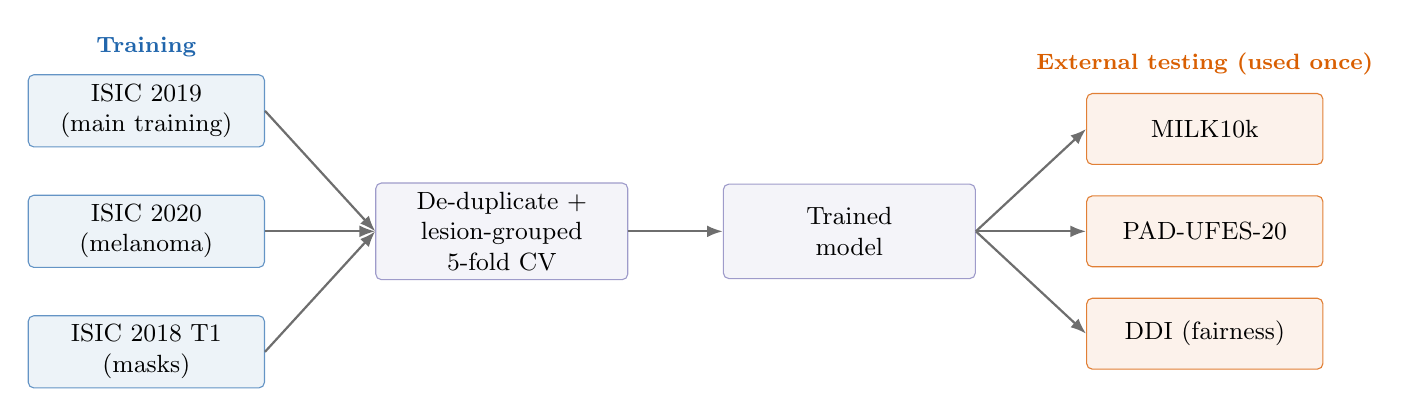
\begin{tikzpicture}[font=\small, node distance=6mm and 9mm,
  tr/.style={draw=hcBlue!70,fill=hcBlue!8,rounded corners=2pt,minimum width=30mm,minimum height=9mm,align=center},
  te/.style={draw=hcOrange!80,fill=hcOrange!8,rounded corners=2pt,minimum width=30mm,minimum height=9mm,align=center},
  md/.style={draw=hcPurple!70,fill=hcPurple!8,rounded corners=2pt,minimum width=32mm,minimum height=12mm,align=center},
  fl/.style={-{Latex[length=2mm]},draw=hcGray,thick}]
\node[tr] (a) {ISIC 2019\\(main training)};
\node[tr,below=of a] (b) {ISIC 2020\\(melanoma)};
\node[tr,below=of b] (c) {ISIC 2018 T1\\(masks)};
\node[md,right=14mm of b] (m) {De-duplicate +\\lesion-grouped\\5-fold CV};
\node[md,right=12mm of m] (mod) {Trained\\model};
\node[te,right=14mm of mod,yshift=13mm] (x) {MILK10k};
\node[te,right=14mm of mod] (y) {PAD-UFES-20};
\node[te,right=14mm of mod,yshift=-13mm] (z) {DDI (fairness)};
\draw[fl] (a.east)--(m.west); \draw[fl] (b.east)--(m.west); \draw[fl] (c.east)--(m.west);
\draw[fl] (m)--(mod);
\draw[fl] (mod.east)--(x.west); \draw[fl] (mod.east)--(y.west); \draw[fl] (mod.east)--(z.west);
\node[above=1mm of a,font=\footnotesize\bfseries,text=hcBlue] {Training};
\node[above=1mm of x,font=\footnotesize\bfseries,text=hcOrange] {External testing (used once)};
\end{tikzpicture}
\caption{How the recommended datasets are used: training data are
cleaned and split by lesion; external sets are used only once, for the
final evaluation.}
\label{fig:flow}
\end{figure}

% =====================================================================
\section{Download Links and Licences}
\begin{table}[H]
\centering
\caption{Where to obtain each recommended dataset.}
\renewcommand{\arraystretch}{1.25}
\small
\begin{tabularx}{\linewidth}{@{}L{2.6cm} L{2.6cm} Y@{}}
\toprule
\textbf{Dataset} & \textbf{Licence} & \textbf{Access} \\
\midrule
ISIC 2016--2019 & CC-0 / CC BY-NC & \url{https://challenge.isic-archive.com/data/} \\
HAM10000 & CC BY-NC 4.0 & \url{https://doi.org/10.7910/DVN/DBW86T} \\
ISIC 2020 & CC BY-NC 4.0 & \url{https://doi.org/10.34970/2020-ds01} (also on Kaggle) \\
SLICE-3D & CC BY-NC (CC BY subset) & \url{https://doi.org/10.34970/2024-slice-3d} \\
MILK10k & CC BY-NC & \url{https://doi.org/10.34970/648456} \\
BCN20000 & CC BY 4.0 & \url{https://doi.org/10.6084/m9.figshare.24140028} \\
PAD-UFES-20 & CC BY 4.0 & \url{https://doi.org/10.17632/zr7vgbcyr2.1} \\
DDI & Research-use agreement & Stanford AIMI shared datasets portal \\
Fitzpatrick 17k & CC BY-NC-SA 3.0 & \url{https://github.com/mattgroh/fitzpatrick17k} \\
PH2 & Research use & \url{https://www.fc.up.pt/addi/ph2\%20database.html} \\
\bottomrule
\end{tabularx}
\end{table}
All recommended licences allow academic research. Most forbid
commercial use; for a commercial product, only the CC BY sets
(BCN20000, PAD-UFES-20, SLICE-3D permissive subset) are usable without
further agreements.

% =====================================================================
\section{Pitfalls and Good Practice}
\begin{enumerate}
  \item \textbf{Remove duplicates across datasets} using a perceptual
        image hash before any split~\cite{cassidy2022isic}. ISIC~2018
        Task~3 = HAM10000; ISIC~2019 $\supset$ HAM10000 + BCN20000;
        MILK10k shares some ISIC images. Whether ISIC~2019 and ISIC~2020
        overlap could not be confirmed, so check this with a hash as well.
  \item \textbf{Split by lesion or patient}, never by image
        (\texttt{GroupKFold} on \texttt{lesion\_id} or
        \texttt{patient\_id}).
  \item \textbf{Report balanced accuracy and per-class sensitivity},
        not only accuracy, because prevalence varies from 0.1\% to 47\%.
  \item \textbf{Report results per skin type} on DDI and PAD-UFES-20.
  \item \textbf{Keep external test sets untouched} until the final
        evaluation. Tuning on them is a form of leakage.
  \item \textbf{Harmonize labels} when combining datasets: map
        AKIEC/AK/ACK to one class and SCC/SCCKA to one class, and keep a
        written mapping table in the project repository.
\end{enumerate}

\keybox{\textbf{Summary:} train on ISIC~2019 + ISIC~2020 (segmentation on
ISIC~2018), test externally on MILK10k and PAD-UFES-20, test fairness on
DDI, and always de-duplicate and split by lesion.}

\bibliographystyle{IEEEtran}
\bibliography{references}
\end{document}
